\documentclass[border=10pt]{standalone}
\usepackage{tikz}
\usetikzlibrary{calc,arrows.meta,positioning}

% Colors matching the lecture notes
\usepackage{xcolor}
\definecolor{my_blue}{RGB}{0,114,178}
\definecolor{my_red}{RGB}{213,94,0}
\definecolor{my_green}{RGB}{0,158,115}

% Node styles matching the lecture notes
\tikzset{
  neuron/.style     = {circle, draw=black!50, very thick, minimum size=8.5mm},
  inputnode/.style  = {neuron, fill=my_green!90},
  hiddennode/.style = {neuron, fill=my_blue!90},
  outputnode/.style = {neuron, fill=my_red!85},
  conn/.style       = {gray!70, -{Latex[length=2.2mm,width=1.4mm]}, line width=0.5pt},
  lbl/.style        = {font=\small},
  biglbl/.style     = {font=\normalsize\bfseries}
}

\begin{document}
% TikZ picture: Two-hidden-layer (DNN) architecture with two output nodes (top: ŷ₁, bottom: ŷ₂)
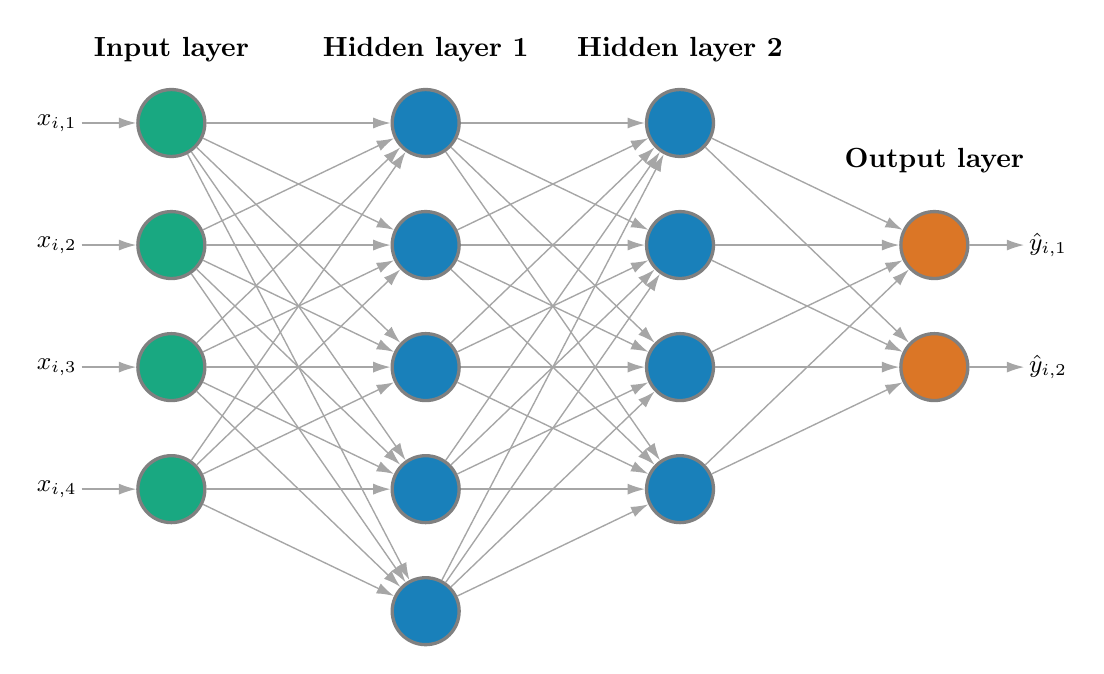
\begin{tikzpicture}[x=1.9cm, y=1.55cm]
    % Layer sizes
    \def\nIn{4}     % input neurons
    \def\nHone{5}   % first hidden layer
    \def\nHtwo{4}   % second hidden layer
    \def\nOut{2}    % output neurons

    % Vertical centering (integer-safe)
    \pgfmathtruncatemacro{\yminIn}{-(\nIn-1)/2}
    \pgfmathtruncatemacro{\yminHone}{-(\nHone-1)/2}
    \pgfmathtruncatemacro{\yminHtwo}{-(\nHtwo-1)/2}
    \pgfmathtruncatemacro{\yminOut}{-(\nOut-1)/2}

    % X positions
    \coordinate (Xin)  at (0,0);
    \coordinate (Xh1)  at (1.7,0);
    \coordinate (Xh2)  at (3.4,0);
    \coordinate (Xout) at (5.1,0);

    % ----- Input layer -----
    \foreach \i in {1,...,\nIn}{
      \node[inputnode] (I\i) at ($(Xin)+(0,\yminIn+\i-1)$) {};
      \pgfmathtruncatemacro{\lab}{\nIn - \i + 1}
      \node[lbl,left=18pt of I\i] {$x_{i,\lab}$};
      \draw[conn] ($(I\i)+(-0.6,0)$) -- (I\i);
    }
    \node[biglbl,above=6pt of I\nIn] {Input layer};

    % ----- Hidden layer 1 -----
    \foreach \h in {1,...,\nHone}{
      \node[hiddennode] (Hone\h) at ($(Xh1)+(0,\yminHone+\h-1)$) {};
    }
    \node[biglbl,above=6pt of Hone\nHone] {Hidden layer 1};

    % Connections: input → hidden 1
    \foreach \i in {1,...,\nIn}{
      \foreach \h in {1,...,\nHone}{
        \draw[conn] (I\i) -- (Hone\h);
      }
    }

    % ----- Hidden layer 2 -----
    \foreach \h in {1,...,\nHtwo}{
      \node[hiddennode] (Htwo\h) at ($(Xh2)+(0,\yminHtwo+\h-1)$) {};
    }
    \node[biglbl,above=6pt of Htwo\nHtwo] {Hidden layer 2};

    % Connections: hidden 1 → hidden 2
    \foreach \h in {1,...,\nHone}{
      \foreach \k in {1,...,\nHtwo}{
        \draw[conn] (Hone\h) -- (Htwo\k);
      }
    }

    % ----- Output layer (reversed order so ŷ₁ is top, ŷ₂ bottom) -----
    \foreach \o [evaluate=\o as \rev using int(\nOut-\o+1)] in {1,...,\nOut}{
      \node[outputnode] (O\rev) at ($(Xout)+(0,\yminOut+\o-1)$) {};
      \node[lbl,right=18pt of O\rev] {$\hat{y}_{i,\rev}$};
      % arrow from node → label
      \draw[conn] (O\rev) -- ($(O\rev)+(0.6,0)$);
    }
    \node[biglbl,above=10pt of O1] {Output layer};

    % Connections: hidden 2 → outputs
    \foreach \h in {1,...,\nHtwo}{
      \foreach \o in {1,...,\nOut}{
        \draw[conn] (Htwo\h) -- (O\o);
      }
    }
\end{tikzpicture}
\end{document}


